\chapter{适应性免疫与疫苗接种}\label{ch:b3:adaptive-immunity}

1796 年，一位乡村医生从一名挤奶女工的牛痘疮口上刮取脓液，
将其接种到一名男孩的手臂上，六周后又给他接种天花；
这名男孩未曾发病。1980 年，世界卫生组织
宣布天花——这种疾病在二十世纪曾造成三亿人死亡——
已借助该方法在地球上被根除。
詹纳在不知情的情况下调动的那套系统，
能够识别从未接触过的任何分子，从一千亿种
受体中挑出少数与之相配者，并使携带它们的细胞
在一周内增殖百万倍，并在此过程中借突变与选择
改善其匹配度，并将结果记忆终生；它
还学会不攻击产生它的机体，而其学习失败
便是\omterm{def:b3:adaptive-immunity:tolerance}{自身免疫}病。本章讨论\omterm{def:b3:adaptive-immunity:lymphocytes}{淋巴细胞}，
它们受体的形成方式，免疫应答的产生与记忆，
\omterm{def:b3:adaptive-immunity:tolerance}{耐受}的建立与丧失，
以及足够多的人接种\omterm{def:b3:adaptive-immunity:vaccine}{疫苗}后保护未接种者的
计算原理。

\section{淋巴细胞与克隆选择}

\begin{definition}[淋巴细胞及其受体]\label{def:b3:adaptive-immunity:lymphocytes}
\index{淋巴细胞}\index{B 细胞}\index{T 细胞}\index{抗原}\index{克隆选择}\index{淋巴结}
\emph{适应性免疫}由\emph{淋巴细胞}承担：\emph{B 细胞}，
在骨髓中成熟，其抗原受体为一种膜结合的
\emph{\omterm{def:b3:adaptive-immunity:antibody}{抗体}}，之后将其分泌出去；以及\emph{T
细胞}，在\omterm{def:b3:adaptive-immunity:tolerance}{胸腺}中成熟，其受体识别
其他细胞表面呈递的肽段。一个
\emph{抗原}是受体所结合的任何物质；实际被接触的部分
即为\emph{表位}。奠基性的事实是\emph{克隆
选择}（伯内特，1957 年）：每个淋巴细胞仅携带一种专一性的受体，
且该专一性在接触任何抗原之前即已确定；机体拥有
由约 $10^{11}$ 个此类细胞构成的库；抗原选出
其受体与之相配的少数细胞，并促使其增殖，形成由效应细胞
与\omterm{def:b3:adaptive-immunity:response}{记忆细胞}组成的克隆；而其受体与机体自身分子相配的淋巴细胞
在成熟过程中被清除或沉默。这些细胞
不断在血液与\emph{淋巴结}之间循环，
脾脏及黏膜淋巴组织，在此处由\omterm{def:b3:innate-immunity:innate}{树突状细胞}（见
\cref{ch:b3:innate-immunity}）携带的抗原被呈递，使稀有的
对应细胞——对某一给定表位而言约为十万分之一——
在一两天之内便能找到它。
\end{definition}

\begin{proof}[证据]
诺萨尔与莱德伯格（1958 年）将来自免疫大鼠的单个\omterm{def:b3:adaptive-immunity:lymphocytes}{淋巴细胞}
置于微滴中，检测每个细胞分泌的\omterm{def:b3:adaptive-immunity:antibody}{抗体}：每个
细胞只产生针对两种\omterm{def:b3:adaptive-immunity:lymphocytes}{抗原}之一的\omterm{def:b3:adaptive-immunity:antibody}{抗体}，绝不同时针对两者。伯内特
在前一年便已作出预测。利根川进（1976 年）比较了
胚胎细胞与分泌\omterm{def:b3:adaptive-immunity:antibody}{抗体}的\omterm{def:b3:cancer-biology:hallmarks}{肿瘤}细胞中\omterm{def:b3:adaptive-immunity:antibody}{抗体}基因的
DNA：在胚胎中，可变区与恒定区相距甚远，而在
\omterm{def:b3:cancer-biology:hallmarks}{肿瘤}中二者已相连——该基因在体细胞中已被切割并拼接，
这是首次证明基因组会被有目的地重排的
证据。
\end{proof}

\section{制造一千亿种受体}

\begin{definition}[抗体结构与 V(D)J 重组]\label{def:b3:adaptive-immunity:antibody}
\index{抗体}\index{免疫球蛋白}\index{V(D)J 重组}\index{RAG}\index{连接多样性}\index{类别转换}
\emph{抗体}（即免疫球蛋白）由两条相同的重链和
两条相同的轻链组成，每条链末端为\emph{可变区}结构域，
其后为\emph{恒定区}结构域；两条臂各自结合一个
表位，依靠重链与轻链可变区各三个超变环结合；
茎部（Fc）则是吞噬细胞、
\omterm{def:b3:innate-immunity:complement}{补体}和肥大细胞识别的部位。五类抗体的区别在于其
重链恒定区：IgM，最先产生，为五聚体，
能很好地激活\omterm{def:b3:innate-immunity:complement}{补体}；IgG 是血液和组织中的主力，
可穿过胎盘；IgA 为二聚体，经黏膜表面
分泌进入肠道、气道和乳汁；IgE 与肥大细胞结合，针对
蠕虫，也是过敏的病因；IgD。可变区结构域并不
以此形式直接编码。重链基因座约含 $40$ 个有功能的
\emph{V} 片段、$25$ 个 \emph{D} 片段和 $6$ 个 \emph{J} 片段；发育中的 B~细胞
各选一个，通过\emph{V(D)J 重组}将它们连接：
RAG1 与 RAG2 两种酶在位于片段两侧的重组信号序列处切割，
片段末端借助\omterm{def:b3:dna-repair:dsb}{非同源末端连接}
机制完成连接（见\cref{ch:b3:dna-repair}），各连接处的核苷酸
会被随机修剪和添加（由 TdT 酶完成）——\emph{连接
多样性}，恰好位于第三个超变环中。
轻链以 V 和 J 片段进行同样的重组。免疫应答开始后，
同一可变区通过第二次重排与另一恒定区相连，
这一过程称为\emph{类别转换}，改变抗体的
功能而不改变其专一性。
\end{definition}

\begin{theorem}[受体库的大小]\label{thm:b3:adaptive-immunity:repertoire}
\index{受体库!组合性}
设重链片段 $V_{H} = 40$、$D = 25$、$J_{H} = 6$，轻链
来自两个基因座，其 $(V_{\kappa}, J_{\kappa}) = (40, 5)$ 与
$(V_{\lambda}, J_{\lambda}) = (30, 4)$，仅由片段选择可得的
不同重链–轻链组合数为
\[
(40\times 25\times 6)\times(40\times 5 + 30\times 4) = 6000\times 320
= 1.9\times 10^{6}.
\]
两个重链连接处与一个轻链连接处的\omterm{def:b3:adaptive-immunity:antibody}{连接多样性}，
使此数再乘以量级为 $10^{4}$--$10^{5}$ 的因子，得到
潜在受体库超过 $10^{10}$，由不到 $200$ 个基因
片段产生——超过机体内 B~细胞的数目，故实际
受体库只是可能受体库的一个样本。\omterm{def:b3:adaptive-immunity:germinal-centre}{体细胞
高频突变}在应答期间（见下文）为
每个被选中的受体生成变体。
\end{theorem}
\begin{proof}
每条重链由一个 V、一个 D 和一个 J 组成；每条轻链由一个 V 和
一个 J 组成，取自两个基因座之一；任一重链与任一轻链配对，故计数
相乘（乘法原理），两个轻链基因座则相加。
连接因子即随机修剪与添加在一个连接处能产生的不同序列数
——每个连接处至少有几十种——
再取连接数的幂；其确切值
未作定义，但三个连接处各有 $30$--$50$ 种结果时，得出
$3\times 10^{4}$ 至 $10^{5}$。\omterm{def:b3:adaptive-immunity:mhc}{T~细胞受体}的计数中，两条链以相同方式重排，
且\omterm{def:b3:adaptive-immunity:antibody}{连接多样性}的贡献更大，
数量级与此相同。
\end{proof}

\begin{omfigure}
\begin{tikzpicture}[every node/.style={font=\scriptsize}, >=stealth]
  % antibody Y
  \begin{scope}[xshift=0cm]
    % heavy chains
    \draw[very thick, omDef] (0,0) -- (0,1.6) -- (-1.3,3.0); \draw[very thick, omDef] (0.35,0) -- (0.35,1.6) -- (1.65,3.0);
    % light chains
    \draw[very thick, omProp] (-0.45,1.55) -- (-1.75,2.95); \draw[very thick, omProp] (0.8,1.55) -- (2.1,2.95);
    \fill[omThm] (-1.55,3.0) circle (0.12); \fill[omThm] (1.9,3.0) circle (0.12);
    \node[above, align=center] at (-1.5,3.15) {可变区：\\抗原结合位点}; 
    \node[right, align=left] at (0.55,0.5) {Fc 茎（恒定区）：\\类别决定功能};
    \node[left, omProp] at (-0.7,2.1) {轻链}; \node[right, omDef] at (0.4,1.3) {重链};
    \draw[omDef] (0.05,1.1) -- (0.3,1.1); \draw[omDef] (0.05,0.7) -- (0.3,0.7);
  \end{scope}
  % V(D)J locus
  \begin{scope}[xshift=4.2cm, yshift=2.4cm, xscale=0.86]
    \draw[very thick, gray] (0,0) -- (8.2,0);
    \foreach \x in {0.2,0.6,1.0,1.4} \draw[thick, fill=omDef!40] (\x,-0.15) rectangle (\x+0.3,0.15);
    \node[above] at (0.95,0.2) {V 片段（$\sim 40$）}; \node[font=\tiny] at (1.95,0) {$\cdots$};
    \foreach \x in {2.5,2.8,3.1} \draw[thick, fill=omProp!50] (\x,-0.15) rectangle (\x+0.2,0.15);
    \node[above] at (2.9,0.2) {D（$25$）};
    \foreach \x in {3.8,4.1,4.4} \draw[thick, fill=omMeth!50] (\x,-0.15) rectangle (\x+0.2,0.15);
    \node[above] at (4.2,0.2) {J（$6$）};
    \foreach \x/\lab in {5.3/\mu,6.0/\delta,6.7/\gamma,7.4/\alpha} { \draw[thick, fill=gray!30] (\x,-0.15) rectangle (\x+0.5,0.15); \node[above] at (\x+0.25,0.2) {C$_{\lab}$}; }
    \draw[->, thick] (4.1,-0.4) -- (4.1,-1.1) node[midway, right, align=left, font=\tiny] {RAG 在信号序列处切割；一个 V、一个 D、\\一个 J 被连接，TdT 加入随机核苷酸};
    % rearranged
    \draw[very thick, gray] (0,-1.5) -- (3.3,-1.5);
    \draw[thick, fill=omDef!40] (1.0,-1.65) rectangle (1.3,-1.35); \fill[omThm] (1.3,-1.65) rectangle (1.4,-1.35);
    \draw[thick, fill=omProp!50] (1.4,-1.65) rectangle (1.6,-1.35); \fill[omThm] (1.6,-1.65) rectangle (1.7,-1.35);
    \draw[thick, fill=omMeth!50] (1.7,-1.65) rectangle (1.9,-1.35);
    \draw[thick, fill=gray!30] (2.6,-1.65) rectangle (3.1,-1.35); \node[above] at (2.85,-1.3) {C$_{\mu}$};
    \node[below, align=center] at (1.45,-1.7) {VDJ 连接：可变区，\\红色：连接处核苷酸};
    \node[right, align=left, font=\tiny] at (3.4,-2.0) {与 C$_{\mu}$ 拼接：IgM 重链；\\类别转换之后，同一 \\VDJ 与 C$_{\gamma}$ 或 C$_{\alpha}$ 连接};
  \end{scope}
\end{tikzpicture}

{\small 左：\omterm{def:b3:adaptive-immunity:antibody}{抗体}——两条重链与两条轻链，两端的可变区形成两个结合位点，
恒定的茎部由免疫系统其余部分识别。右：
重链基因座在 V(D)J 重组前后的情况，
重组时每类片段各选取一个，
并在连接处加入随机核苷酸。}
\end{omfigure}

\begin{definition}[T~细胞受体与 MHC]\label{def:b3:adaptive-immunity:mhc}
\index{T~细胞受体}\index{主要组织相容性复合体}\index{抗原提呈}\index{MHC 限制性}\index{HLA}
\emph{T~细胞受体}是由同样重组过程构建的双链分子，
从不分泌，也不与游离于溶液中的\omterm{def:b3:adaptive-immunity:lymphocytes}{抗原}结合：
它识别的是位于另一细胞表面的
\emph{主要组织相容性复合体}（MHC）分子凹槽中所载的短肽。
\emph{MHC~I 类分子}存在于每个有核细胞上，展示
由蛋白酶体从细胞自身胞质蛋白中切下的 8 至 10 个残基的肽段，
它是细胞正在合成之物的样本，包括任何\omterm{def:b3:virology:virus}{病毒}——
提呈给 \emph{CD8} T~细胞，若该肽为外来的，
则这些细胞杀伤该细胞。\emph{MHC~II 类分子}存在于\omterm{def:b3:innate-immunity:innate}{树突状细胞}、
\omterm{def:b3:innate-immunity:innate}{巨噬细胞}和 B~细胞上，展示 13 至 25 个残基的肽段，
来源于细胞摄取并在\omterm{def:b3:membrane-traffic:endocytosis}{内体}中消化的蛋白质，
提呈给 \emph{CD4} T~细胞；后者通过辅助作用予以应答。T~细胞是
\emph{限制性的}：它只在其被选定的 MHC 等位基因上识别其肽段。
MHC 基因（人类中称 \emph{HLA}）是基因组中多态性最高的一类，
有数千个等位基因，彼此在凹槽上存在差异，
因此每个人对每种蛋白质所展示的肽段样本各不相同，
没有任何病原体能在所有人中逃避提呈，
同时，来自不匹配供体的移植器官会
被受者的大部分 T~细胞识别为外来物。
\end{definition}

\begin{proof}[证据]
津克纳格尔与多尔蒂（1974）用\omterm{def:b3:virology:virus}{病毒}感染两个近交系小鼠，
并用其细胞毒性 T~细胞检测被感染的靶细胞：
尽管\omterm{def:b3:virology:virus}{病毒}相同，T~细胞只杀伤同品系的被感染细胞，
而不杀伤另一品系的。T~细胞仅在与自身 MHC 分子共同出现时才识别\omterm{def:b3:virology:virus}{病毒}——
即 \emph{MHC 限制性}——这一现象后来得到解释：
比约克曼（1987）解析了一个 MHC 分子的晶体结构，
显示其凹槽中有一个肽，
\omterm{def:b3:adaptive-immunity:mhc}{T~细胞受体}也被证明同时结合两者。
\end{proof}

\begin{omfigure}
\begin{tikzpicture}[every node/.style={font=\scriptsize}, >=stealth]
  % class I pathway
  \begin{scope}
    \draw[thick, omDef, fill=omDef!8] (0,0) rectangle (6.2,3.6); \node[anchor=north west] at (0.05,3.55) {任一有核细胞};
    \node[draw, rounded corners, fill=omThm!20, font=\tiny, align=center] (v) at (1.4,2.6) {病毒或自身蛋白 \\位于胞质中};
    \node[draw, rounded corners, fill=gray!20, font=\tiny, align=center] (p) at (1.4,1.5) {蛋白酶体：\\8--10 个残基的肽};
    \node[draw, rounded corners, fill=omDef!25, font=\tiny, align=center] (er) at (4.6,1.5) {内质网：装载到 \\MHC~I 类分子上};
    \draw[->, thick] (v) -- (p); \draw[->, thick] (p) -- node[midway, above, font=\tiny] {TAP} (er);
    \draw[->, thick] (er) -- (4.6,3.55);
    \draw[thick, fill=omDef!40] (4.4,3.6) rectangle (4.8,4.1); \fill[omThm] (4.6,4.2) circle (0.09);
    \node[above, align=center] at (4.6,4.35) {肽--MHC~I\\被 CD8 T 细胞识别：杀伤};
  \end{scope}
  % class II pathway
  \begin{scope}[xshift=7.2cm]
    \draw[thick, omProp, fill=omProp!8] (0,0) rectangle (6.2,3.6); \node[anchor=north west] at (0.05,3.55) {树突状细胞、巨噬细胞、B 细胞};
    \node[draw, rounded corners, fill=omThm!20, font=\tiny, align=center] (ex) at (1.4,2.6) {摄取的蛋白质 \\进入内体};
    \node[draw, rounded corners, fill=gray!20, font=\tiny, align=center] (dig) at (1.4,1.5) {消化：\\13--25 个残基的肽};
    \node[draw, rounded corners, fill=omProp!30, font=\tiny, align=center] (m2) at (4.6,1.5) {MHC~II 类分子 \\在此装载};
    \draw[->, thick] (ex) -- (dig); \draw[->, thick] (dig) -- (m2);
    \draw[->, thick] (m2) -- (4.6,3.55);
    \draw[thick, fill=omProp!50] (4.4,3.6) rectangle (4.8,4.1); \fill[omThm] (4.6,4.2) circle (0.09);
    \node[above, align=center] at (4.6,4.35) {肽--MHC~II\\被 CD4 T 细胞识别：辅助};
  \end{scope}
\end{tikzpicture}

{\small 两条提呈途径。I 类分子向 CD8 T~细胞展示
细胞自身正在合成的内容；II 类分子向 CD4 T~细胞展示
\omterm{def:b3:adaptive-immunity:mhc}{抗原提呈}细胞所吞噬的内容。细胞毒性应答针对
前者，辅助性应答针对后者。}
\end{omfigure}

\section{应答}

\begin{definition}[激活、辅助与杀伤]\label{def:b3:adaptive-immunity:response}
\index{辅助性 T 细胞}\index{细胞毒性 T 细胞}\index{共刺激}\index{调节性 T 细胞}\index{浆细胞}\index{记忆细胞}
初始 T~细胞的受体与\omterm{def:b3:innate-immunity:innate}{树突状细胞}上的肽--MHC 结合时，即被激活，
该\omterm{def:b3:innate-immunity:innate}{树突状细胞}同时提供共刺激（\cref{ch:b3:innate-immunity}）；
随后每 6--8 小时分裂一次，持续一周，并发生分化。
\emph{CD4 辅助性} T~细胞依据\omterm{def:b3:innate-immunity:innate}{树突状细胞}所分泌的\omterm{def:b3:innate-immunity:inflammation}{细胞因子}
分化为若干亚群：Th1，可活化\omterm{def:b3:innate-immunity:innate}{巨噬细胞}，使其杀灭所吞噬的病原（结核病）；
Th2，驱动 IgE 产生及嗜酸性粒细胞作用，以对抗蠕虫；
Th17，招募\omterm{def:b3:innate-immunity:innate}{中性粒细胞}，对抗胞外细菌和真菌；
滤泡辅助性 T~细胞，帮助 B~细胞；
以及\emph{调节性} T~细胞，起抑制作用。\emph{CD8 细胞毒性} T~细胞
杀伤在 I 类分子上展示其肽段的细胞，杀伤方式为穿孔素、颗粒酶，
以及 Fas 配体，诱导\omterm{def:b3:cell-cycle-apoptosis:apoptosis}{细胞凋亡}
（\cref{ch:b3:cell-cycle-apoptosis}）——是抗\omterm{def:b3:virology:virus}{病毒}与
抗\omterm{def:b3:cancer-biology:hallmarks}{肿瘤}的防线。B~细胞由\omterm{def:b3:adaptive-immunity:lymphocytes}{抗原}与其受体结合，并
获得滤泡辅助性 T~细胞的帮助，该 T~细胞识别同一\omterm{def:b3:adaptive-immunity:lymphocytes}{抗原}
在 B~细胞 II~类分子上的肽段；随后成为\emph{浆细胞}，
每秒分泌数千个\omterm{def:b3:adaptive-immunity:antibody}{抗体}，持续数天（短寿命，位于\omterm{def:b3:adaptive-immunity:lymphocytes}{淋巴结}中），
或持续数年（长寿，位于骨髓中），或进入\omterm{def:b3:adaptive-immunity:germinal-centre}{生发中心}。
\emph{记忆} B~细胞与 T~细胞——长寿，数量多于初始前体细胞，
且应答更快——是每次应答后的遗留，
也是\omterm{def:b3:adaptive-immunity:vaccine}{疫苗}接种的基础。
\end{definition}

\begin{definition}[生发中心]\label{def:b3:adaptive-immunity:germinal-centre}
\index{生发中心}\index{体细胞高频突变}\index{亲和力成熟}
在\emph{生发中心}中（一种在应答约一周后于\omterm{def:b3:adaptive-immunity:lymphocytes}{淋巴结}内形成的结构），
被激活的 B~细胞运行一种演化算法。
在其暗区，细胞每 6 小时分裂一次，
其\omterm{def:b3:adaptive-immunity:antibody}{抗体}可变区基因由酶 AID 突变，约每千个碱基对每次分裂
发生一次改变——\emph{体细胞高频突变}，
其速率为基因组突变速率的 100 万倍，作用于约 1 千碱基。
在亮区，每个细胞用其新受体检测滤泡\omterm{def:b3:innate-immunity:innate}{树突状细胞}所持有的\omterm{def:b3:adaptive-immunity:lymphocytes}{抗原}，
并竞争 T~细胞的辅助：结合较强的细胞摄取更多\omterm{def:b3:adaptive-immunity:lymphocytes}{抗原}，
呈递更多，获得更多辅助，
并返回暗区再次分裂；结合较弱或已丧失结合能力的细胞
则通过\omterm{def:b3:cell-cycle-apoptosis:apoptosis}{细胞凋亡}死亡。经过 2--3 周的循环，
存活\omterm{def:b3:adaptive-immunity:antibody}{抗体}的亲和力提高百倍至千倍，
——\emph{亲和力成熟}——而获胜者
以\omterm{def:b3:adaptive-immunity:response}{浆细胞}和\omterm{def:b3:adaptive-immunity:response}{记忆细胞}的形式离开，并同时完成
\omterm{def:b3:adaptive-immunity:antibody}{类别转换}。二次应答更快、更大，由质量更高的
\omterm{def:b3:adaptive-immunity:antibody}{抗体}组成，因为它始于这一经选择、扩增且已完成\omterm{def:b3:adaptive-immunity:antibody}{类别转换}的
群体。
\end{definition}

\begin{omfigure}
\begin{tikzpicture}[every node/.style={font=\scriptsize}, >=stealth]
  \draw[thick, omDef, fill=omDef!12] (0,0) ellipse (2.7 and 1.7); \node[above, omDef!70!black] at (0,1.75) {暗区};
  \draw[thick, omMeth!70!black, fill=omMeth!12] (6.2,0) ellipse (2.7 and 1.7); \node[above, omMeth!60!black] at (6.2,1.75) {亮区};
  \node[align=center] at (0,0.3) {B~细胞每 \qty{6}{h} 分裂一次；\\AID 突变抗体 \\基因，突变率 $10^{-3}$ 每碱基对每次分裂};
  \node[align=center] at (6.2,0.3) {用新受体 \\检测滤泡树突状细胞 \\所持抗原；\\竞争 T~细胞辅助};
  \draw[->, very thick, omProp] (2.4,0.7) .. controls (3.6,1.4) and (4.2,1.4) .. (3.7,0.7); \node[above, omProp] at (3.1,1.45) {突变体离开};
  \draw[->, very thick, omMeth!70!black] (3.7,-0.7) .. controls (4.2,-1.4) and (3.6,-1.4) .. (2.4,-0.7); \node[below, omMeth!70!black] at (3.1,-1.45) {胜者返回，再次分裂};
  \draw[->, thick, omThm] (6.6,-1.6) -- (6.6,-2.3); \node[below, omThm, align=center] at (6.6,-2.3) {失败者：细胞凋亡 \\（多数）};
  \draw[->, thick] (8.9,0) -- (9.5,0); \node[right, align=left] at (9.5,0) {2--3 周后：\\浆细胞（长寿，\\位于骨髓）与 \\记忆 B~细胞；亲和力 \\提高 $100$--$1000\times$，类别已转换};
\end{tikzpicture}

{\small 作为演化机器的\omterm{def:b3:adaptive-immunity:germinal-centre}{生发中心}：暗区中发生突变，
亮区中进行选择，并在两者之间循环，直至
离开的\omterm{def:b3:adaptive-immunity:antibody}{抗体}结合能力远优于进入时的\omterm{def:b3:adaptive-immunity:antibody}{抗体}。}
\end{omfigure}

\begin{example}[应答的动力学]\label{ex:b3:adaptive-immunity:kinetics}
约每 $10^{5}$ 个 B~细胞有一个能结合某一表位，故机体的
$10^{11}$ 个 B~细胞含约 $10^{6}$ 个前体，其中或许约 100 个
在引流\omterm{def:b3:adaptive-immunity:lymphocytes}{淋巴结}中与\omterm{def:b3:adaptive-immunity:lymphocytes}{抗原}相遇。每 8 小时分裂一次，100 个细胞
在一周内增至 $10^{2}\times 2^{21} \approx 2\times 10^{8}$ 个。
\omterm{def:b3:adaptive-immunity:antibody}{抗体}在 4--6 天后出现于血清中，先为 IgM，
约 2 周时达峰值，随后以 3 周的半衰期下降，
IgG 随短寿命\omterm{def:b3:adaptive-immunity:response}{浆细胞}死亡而减少，稳定于长寿骨髓\omterm{def:b3:adaptive-immunity:response}{浆细胞}
可维持数年的水平。再次接触\omterm{def:b3:adaptive-immunity:lymphocytes}{抗原}时，
应答始于 $10^{4}$--$10^{5}$ 个高亲和力\omterm{def:b3:adaptive-immunity:response}{记忆细胞}，它们已
转换为 IgG：\omterm{def:b3:adaptive-immunity:antibody}{抗体}在 2 天内升高，高出 10 至 100 倍，
并在病原体立足之前将其中和
——这正是\omterm{def:b3:adaptive-immunity:vaccine}{疫苗}所带来的保护。
\end{example}

\begin{omfigure}
\begin{tikzpicture}
\begin{axis}[
  width=0.7\linewidth, height=5.6cm,
  axis x line=bottom, axis y line=left,
  xmin=0, xmax=70, ymin=1, ymax=10000, ymode=log,
  xlabel={天}, ylabel={血清抗体（相对值）},
  xlabel style={font=\small, at={(axis description cs:0.5,-0.12)}, anchor=north}, ylabel style={font=\small},
  tick label style={font=\small}, xtick={0,10,20,30,40,50,60,70},
  clip=false,
]
\addplot[very thick, omDef, domain=0:40, samples=60] {1 + 100*exp(-((x-14)/5)^2) + 15*(1-exp(-x/10))*exp(-(x-14)/60)*(x>14)};
\addplot[very thick, omThm, domain=40:70, samples=60] {1 + 2500*exp(-((x-48)/5)^2) + 400*(1-exp(-(x-40)/4))*(x>40)};
\draw[->, thick, gray] (axis cs:0,0.6) -- (axis cs:0,1.8); \node[font=\scriptsize, gray, anchor=south west] at (axis cs:0.5,1.3) {首次接触};
\draw[->, thick, gray] (axis cs:40,0.6) -- (axis cs:40,1.8); \node[font=\scriptsize, gray, anchor=south west] at (axis cs:40.5,1.3) {再次接触};
\node[font=\scriptsize, omDef, anchor=south west] at (axis cs:2,600) {初次应答：先 IgM 后 IgG，2 周时达峰值};
\node[font=\scriptsize, omThm, anchor=south east] at (axis cs:69,3500) {再次应答：更快、更高、IgG 为主、亲和力更高};
\end{axis}
\end{tikzpicture}

{\small 初次与再次\omterm{def:b3:adaptive-immunity:antibody}{抗体}应答。第二次接触
始于经扩增、已转换类别并完成\omterm{def:b3:adaptive-immunity:germinal-centre}{亲和力成熟}的\omterm{def:b3:adaptive-immunity:response}{记忆细胞}群，
并在数天内作出应答，其水平是初次应答从未达到的。}
\end{omfigure}

\begin{omfigure}
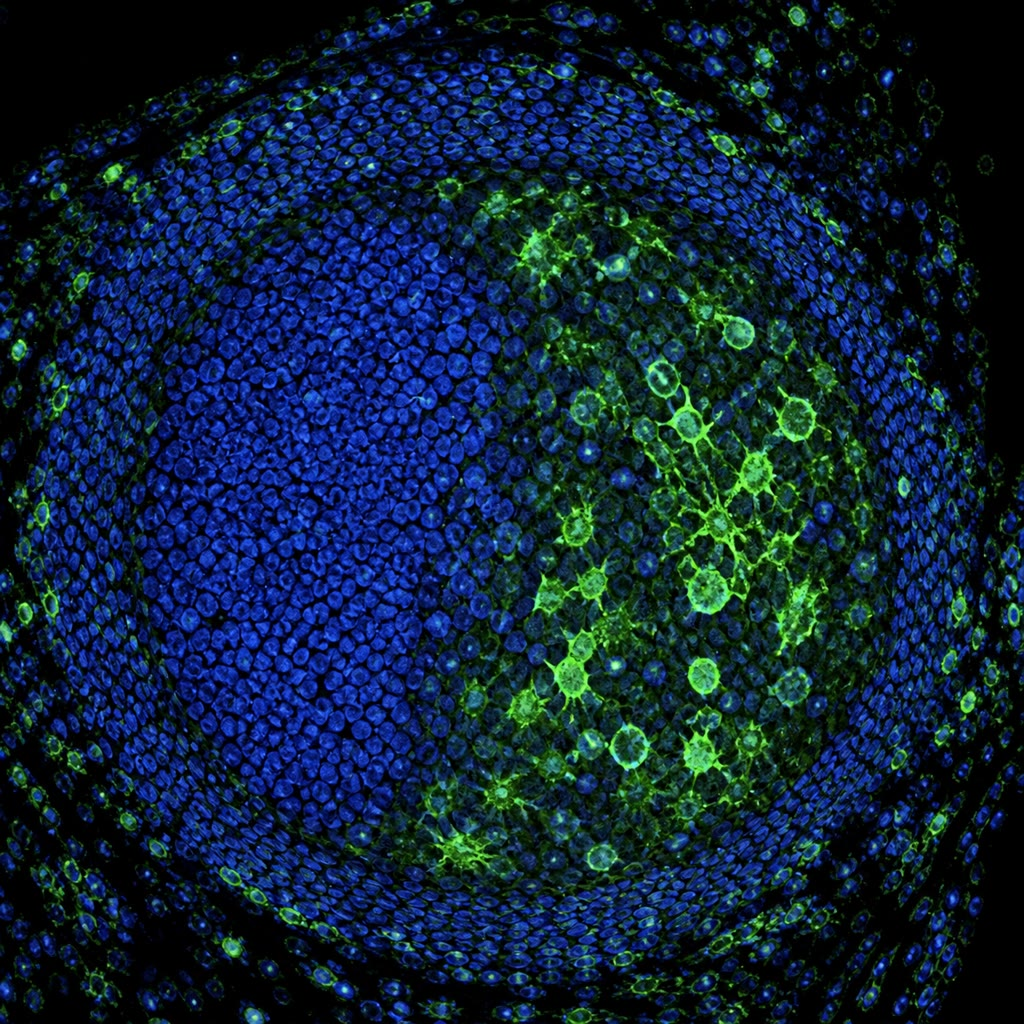
\includegraphics[width=0.36\linewidth]{images/book5/ai/b5-16-germinal-centre.jpg}\hspace{0.04\linewidth}
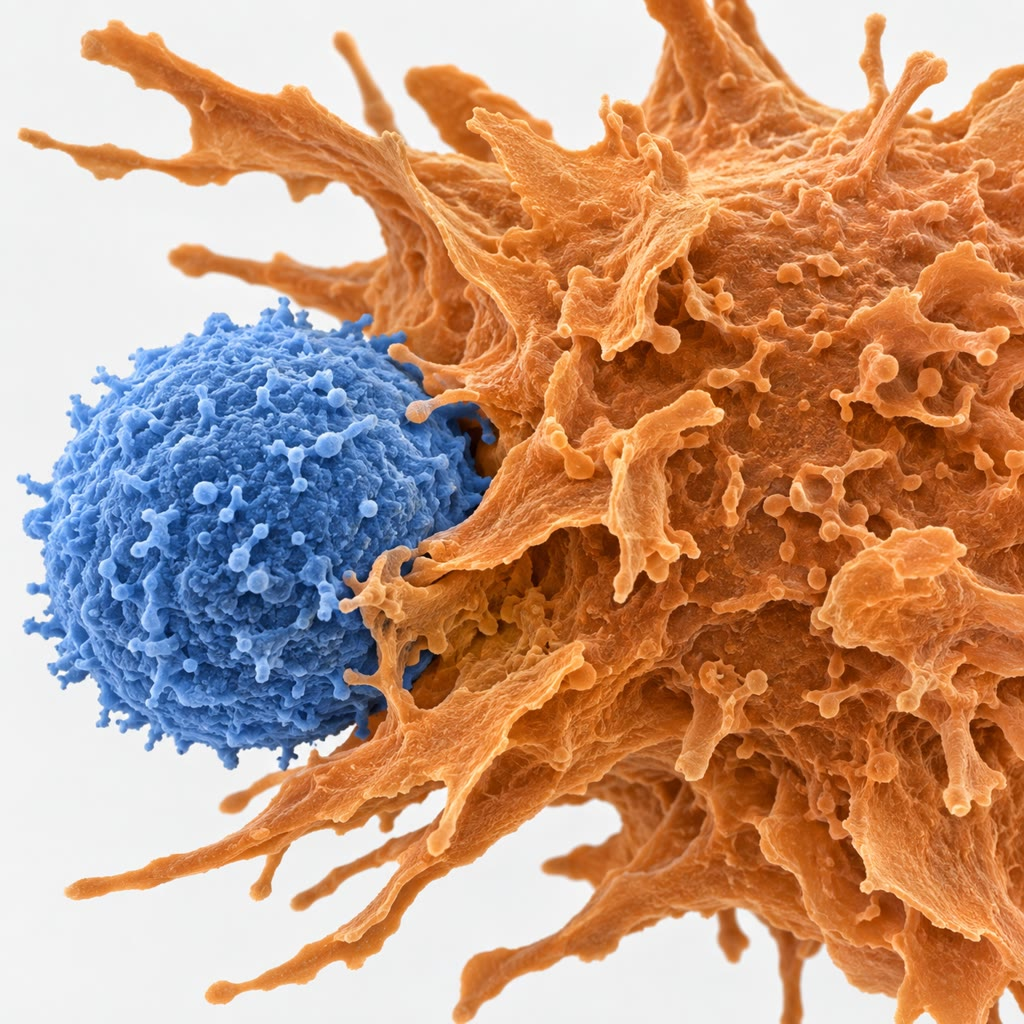
\includegraphics[width=0.36\linewidth]{images/book5/ai/b5-16-t-cell-apc.jpg}

{\small 左：\omterm{def:b3:adaptive-immunity:lymphocytes}{淋巴结}中的\omterm{def:b3:adaptive-immunity:germinal-centre}{生发中心}——拥挤的暗区
与较亮的选择区。右：一个较小的 T~细胞，
与\omterm{def:b3:innate-immunity:innate}{树突状细胞}接触，这一时刻决定了
适应性应答的走向。}
\end{omfigure}

\section{耐受及其失效}

\begin{definition}[耐受]\label{def:b3:adaptive-immunity:tolerance}
\index{耐受}\index{阴性选择}\index{胸腺}\index{无能}\index{FoxP3}\index{自身免疫}
受体库是随机产生的，因此含有识别
自身的受体。\emph{中枢耐受}在细胞成熟时将其清除：
在胸腺中，受体与自身肽--MHC 结合过强的 T~细胞
被杀死（\emph{阴性选择}），完全不能结合 MHC 的
T~细胞同样被杀死（它们毫无用处），只有中间的
少数百分之几得以离开；转录因子 AIRE 使胸腺细胞
表达来自各组织的蛋白质——胰岛素、甲状腺球蛋白——从而
使针对这些蛋白的 T~细胞可在胸腺中被清除。在骨髓中与自身结合的 B~细胞
被清除，或改编其受体。\emph{外周耐受}
处理其余部分：遇到\omterm{def:b3:adaptive-immunity:lymphocytes}{抗原}而缺乏\omterm{def:b3:adaptive-immunity:response}{共刺激}信号的 T~细胞，
则失去应答能力（\emph{无能}），或被清除；此外，
由因子 FoxP3 界定的\emph{调节性} T~细胞，主动
抑制针对自身以及针对食物和\omterm{def:b3:microbiomes:symbiosis}{共生}菌等无害\omterm{def:b3:adaptive-immunity:lymphocytes}{抗原}的应答。
\emph{自身免疫}是这些控制机制的失效：
1 型糖尿病（T~细胞破坏 $\beta$ 细胞）、多发性
硬化症（髓鞘）、类风湿关节炎（关节）、狼疮（针对核成分的
\omterm{def:b3:adaptive-immunity:antibody}{抗体}）、甲状腺疾病；每种疾病都与
特定的 \omterm{def:b3:adaptive-immunity:mhc}{HLA} 等位基因相关，这些等位基因呈递相关的自身肽段，某些
疾病由某种微生物感染引发，该微生物的肽段与
某种自身蛋白相似（链球菌感染后的风湿热）。
\end{definition}

\begin{proof}[证据]
梅达沃（1953）将一个近交系小鼠品系的细胞注入
另一品系的新生小鼠体内；成年后，受者接受了供体品系的皮肤移植物，
而这些移植物在其他情况下本会被排斥，同时
仍排斥来自第三品系的移植物。\omterm{def:b3:adaptive-immunity:tolerance}{耐受}是后天获得的、具有特异性的，
且由免疫系统早期所遇到的\omterm{def:b3:adaptive-immunity:lymphocytes}{抗原}决定——这一实验为
伯内特关于清除自身反应性克隆的理论提供了实验基础。出生时即缺失
功能性 AIRE 基因的儿童会同时对多个器官产生\omterm{def:b3:adaptive-immunity:tolerance}{自身免疫}；
缺乏 \omterm{def:b3:adaptive-immunity:tolerance}{FoxP3} 的儿童（一种罕见的 X 连锁综合征）
在婴儿期即发生致命的\omterm{def:b3:adaptive-immunity:tolerance}{自身免疫}——\omterm{def:b3:adaptive-immunity:tolerance}{耐受}的两个环节，
各自通过其缺失而得以证明。
\end{proof}

\begin{example}[超敏反应、缺陷与移植]\label{ex:b3:adaptive-immunity:failures}
\emph{过敏}是对无害\omterm{def:b3:adaptive-immunity:lymphocytes}{抗原}——花粉、花生、青霉素——发生的 Th2 应答，
产生 IgE；再次接触时，\omterm{def:b3:adaptive-immunity:lymphocytes}{抗原}交联肥大细胞上的 IgE，
使其在数分钟内释放组胺；若\omterm{def:b3:adaptive-immunity:lymphocytes}{抗原}进入血液，
则全身性释放即为
\emph{过敏性休克}，需用肾上腺素治疗。\emph{免疫缺陷}：
缺乏 \omterm{def:b3:adaptive-immunity:antibody}{RAG} 或酶 ADA 的儿童不能产生\omterm{def:b3:adaptive-immunity:lymphocytes}{淋巴细胞}（重症
联合免疫缺陷），若不接受骨髓
移植或基因治疗，便会死于感染；HIV 破坏 CD4 T~细胞，并随之
丧失每一种应答所需的辅助。\emph{移植}：受者的 T~细胞将供者的
\omterm{def:b3:adaptive-immunity:mhc}{HLA} 分子视为异物，多达十分之一的 T~细胞会发生应答——远多于
对任何病原体的应答——因此移植物须在 \omterm{def:b3:adaptive-immunity:mhc}{HLA} 位点上配型，
受者终身需接受免疫抑制；骨髓移植物则
可能转而攻击新宿主。另有一些有意的应用：
\cref{ch:b3:genetic-engineering}中的\omterm{def:b3:genetic-engineering:expression}{单克隆抗体}，
使 T~细胞得以攻击\omterm{def:b3:cancer-biology:hallmarks}{肿瘤}的\omterm{prop:b3:cancer-biology:immune}{检查点抑制剂}
（\cref{ch:b3:cancer-biology}），以及带有针对\omterm{def:b3:cancer-biology:hallmarks}{肿瘤}\omterm{def:b3:adaptive-immunity:lymphocytes}{抗原}的嵌合受体的
工程化 T~细胞（CAR-T），它们治愈了
其他任何疗法都无法奏效的白血病。
\end{example}

\section{接种疫苗}

\begin{definition}[疫苗与群体免疫]\label{def:b3:adaptive-immunity:vaccine}
\index{疫苗}\index{群体免疫}\index{基本再生数}\index{疫苗效力}
\emph{疫苗}呈递病原体的\omterm{def:b3:adaptive-immunity:lymphocytes}{抗原}，借助\omterm{prop:b3:innate-immunity:bridge}{佐剂}或
以能激活固有受体的形式存在，使受种者
在未患病的情况下获得\omterm{def:b3:adaptive-immunity:response}{记忆细胞}和\omterm{def:b3:adaptive-immunity:antibody}{抗体}
（各类疫苗见\cref{ch:b3:virology}）。其\emph{效力}$E$ 为
接种者中获得保护的人所占的比例。保护作用不限于
接种者本人：在一个病原体传播的群体中，每例病例
在所有人都易感时平均感染 $R_{0}$ 人——此数即
\emph{基本再生数}——当部分人已获免疫时，感染人数仅为 $R_{0}$ 乘以
易感者比例，当该数小于 1 时
疫情即会消退。这就是\emph{群体免疫}：免疫者比例超过阈值，
后传播链即被切断，未接种者
——婴儿、免疫缺陷者，以及疫苗未能产生保护的人——
便受到其他人的保护。
\end{definition}

\begin{theorem}[群体免疫阈值]\label{thm:b3:adaptive-immunity:herd}
\index{群体免疫!阈值}\index{SIR 模型}
设群体中比例为 $p$ 的人已获免疫，其余
为易感者，每例病例平均感染 $R_{\text{eff}} = R_{0}(1 -
p)$ 人。若 $R_{\text{eff}} < 1$，则疫情无法开始，也就是
当
\[
p > p_{c} = 1 - \frac{1}{R_{0}} .
\]
对效力为 $E$ 的\omterm{def:b3:adaptive-immunity:vaccine}{疫苗}，所需接种覆盖度为 $f_{c} = p_{c}/E$。
若疫情确在易感群体中发生（SIR 模型，
感染率为 $\beta$，恢复率为 $\gamma$，$R_{0} =
\beta/\gamma$），则当易感者比例降至
$1/R_{0}$ 时达到峰值；从未被感染者的比例 $s_{\infty}$ 满足
$\ln s_{\infty} = -R_{0}(1 - s_{\infty})$.
\end{theorem}
\begin{proof}
每例病例所产生的接触，若所有人都易感，将感染 $R_{0}$ 人；
其中比例为 $1 - p$ 的人易感，故 $R_{\text{eff}} =
R_{0}(1-p)$，由条件 $R_{\text{eff}} < 1$ 得 $p_{c}$；\omterm{def:b3:adaptive-immunity:vaccine}{疫苗}
能保护接种者中比例为 $E$ 的人，使总人口中比例为
$Ef$ 的人获得免疫，故 $Ef > p_{c}$。在 \omterm{thm:b3:adaptive-immunity:herd}{SIR
模型}中，$\mathrm{d}s/\mathrm{d}t = -\beta si$ 与 $\mathrm{d}i/\mathrm{d}t =
\beta si - \gamma i = \gamma i(R_{0}s - 1)$，故 $i$ 在 $s >
1/R_{0}$ 时增长，此后下降：峰值位于 $s = 1/R_{0}$ 处。两式相除，
得 $\mathrm{d}i/\mathrm{d}s = -1 + 1/(R_{0}s)$，故 $i + s -
\ln s/R_{0}$ 为常数；在起点（$s = 1$，$i
\approx 0$）与终点（$i = 0$，$s = s_{\infty}$）处求值，得
$s_{\infty} - \ln s_{\infty}/R_{0} = 1$，即终值关系式。
\end{proof}

\begin{example}[麻疹与天花]\label{ex:b3:adaptive-immunity:measles}
麻疹的 $R_{0} \approx 15$，$p_{c} = 1 - 1/15 = 93\,\%$；若采用
两剂后效力为 $97\,\%$ 的\omterm{def:b3:adaptive-immunity:vaccine}{疫苗}，所需覆盖率为
$96\,\%$——这正是麻疹在接种率稍有下滑时便会卷土重来的原因，
也是未接种\omterm{def:b3:adaptive-immunity:vaccine}{疫苗}的儿童在接种率高的国家中依然安全的原因。
天花的 $R_{0} \approx 5$--$7$，阈值约为
$80$--$85\,\%$，既无动物储库，也无
无症状携带者，且一剂即有效的\omterm{def:b3:adaptive-immunity:vaccine}{疫苗}使其可被根除，并且确已根除。
脊髓灰质炎已近根除。流感与冠状\omterm{def:b3:virology:virus}{病毒}
的\omterm{def:b3:adaptive-immunity:lymphocytes}{抗原}会漂移（\cref{ch:b3:virology}），免疫力也会消退，
二者均不可根除。在未接种\omterm{def:b3:adaptive-immunity:vaccine}{疫苗}的人群中，$R_{0} = 3$ 的疫情
依终值关系式，感染的人口比例为 $1 - s_{\infty} = 94\,\%$；
$R_{0} = 1.5$ 时为 $58\,\%$。
\end{example}

\begin{omfigure}
\begin{tikzpicture}
\begin{axis}[
  width=6.4cm, height=5.4cm,
  axis x line=bottom, axis y line=left,
  xmin=1, xmax=18, ymin=0, ymax=1,
  xlabel={$R_{0}$}, ylabel={阈值 $p_{c}$},
  xlabel style={font=\small, at={(axis description cs:0.5,-0.12)}, anchor=north}, ylabel style={font=\small},
  tick label style={font=\scriptsize}, xtick={1,3,6,9,12,15,18}, ytick={0,0.5,0.8,0.93,1}, yticklabels={0,0.5,0.8,0.93,1},
  clip=false,
]
\addplot[very thick, omDef, domain=1:18, samples=80] {1-1/x};
\fill[omThm] (axis cs:15,0.933) circle (2pt); \node[font=\scriptsize, anchor=south east] at (axis cs:15,0.94) {麻疹};
\fill[omThm] (axis cs:6,0.833) circle (2pt); \node[font=\scriptsize, anchor=north west] at (axis cs:6.3,0.82) {天花};
\fill[omThm] (axis cs:2.5,0.6) circle (2pt); \node[font=\scriptsize, anchor=north west] at (axis cs:2.6,0.58) {1918 年流感};
\end{axis}
\begin{axis}[
  at={(7.6cm,0)}, anchor=south west,
  width=6.4cm, height=5.4cm,
  axis x line=bottom, axis y line=left,
  xmin=0, xmax=60, ymin=0, ymax=0.35,
  xlabel={天}, ylabel={感染者比例},
  xlabel style={font=\small, at={(axis description cs:0.5,-0.12)}, anchor=north}, ylabel style={font=\small},
  tick label style={font=\scriptsize}, xtick={0,20,40,60}, ytick={0,0.1,0.2,0.3},
  clip=false,
]
\addplot[very thick, omThm, smooth] coordinates {(0,0.001) (5,0.003) (10,0.012) (15,0.04) (20,0.12) (25,0.25) (28,0.30) (31,0.27) (35,0.18) (40,0.09) (45,0.04) (50,0.015) (55,0.006) (60,0.002)};
\addplot[very thick, omDef, smooth] coordinates {(0,0.001) (5,0.0015) (10,0.0025) (15,0.004) (20,0.006) (25,0.009) (30,0.012) (35,0.014) (40,0.015) (45,0.014) (50,0.012) (55,0.009) (60,0.007)};
\node[font=\scriptsize, omThm, anchor=west] at (axis cs:30,0.3) {无免疫，$R_{0} = 3$};
\node[font=\scriptsize, omDef, anchor=south west] at (axis cs:32,0.03) {\qty{60}{\%} 已接种：$R_{\text{eff}} = 1.2$};
\end{axis}
\end{tikzpicture}

{\small 左图：阈值 $1 - 1/R_{0}$——疾病传染性越强，
则需要接近全体人口获得免疫。右图：一场 SIR 疫情，
$R_{0} = 3$，分别发生于初始无免疫的人群中，以及 \qty{60}{\%} 已获
免疫的人群中；后者虽不足以遏制疫情，但能使其曲线趋平、进程放缓。}
\end{omfigure}

\begin{omfigure}
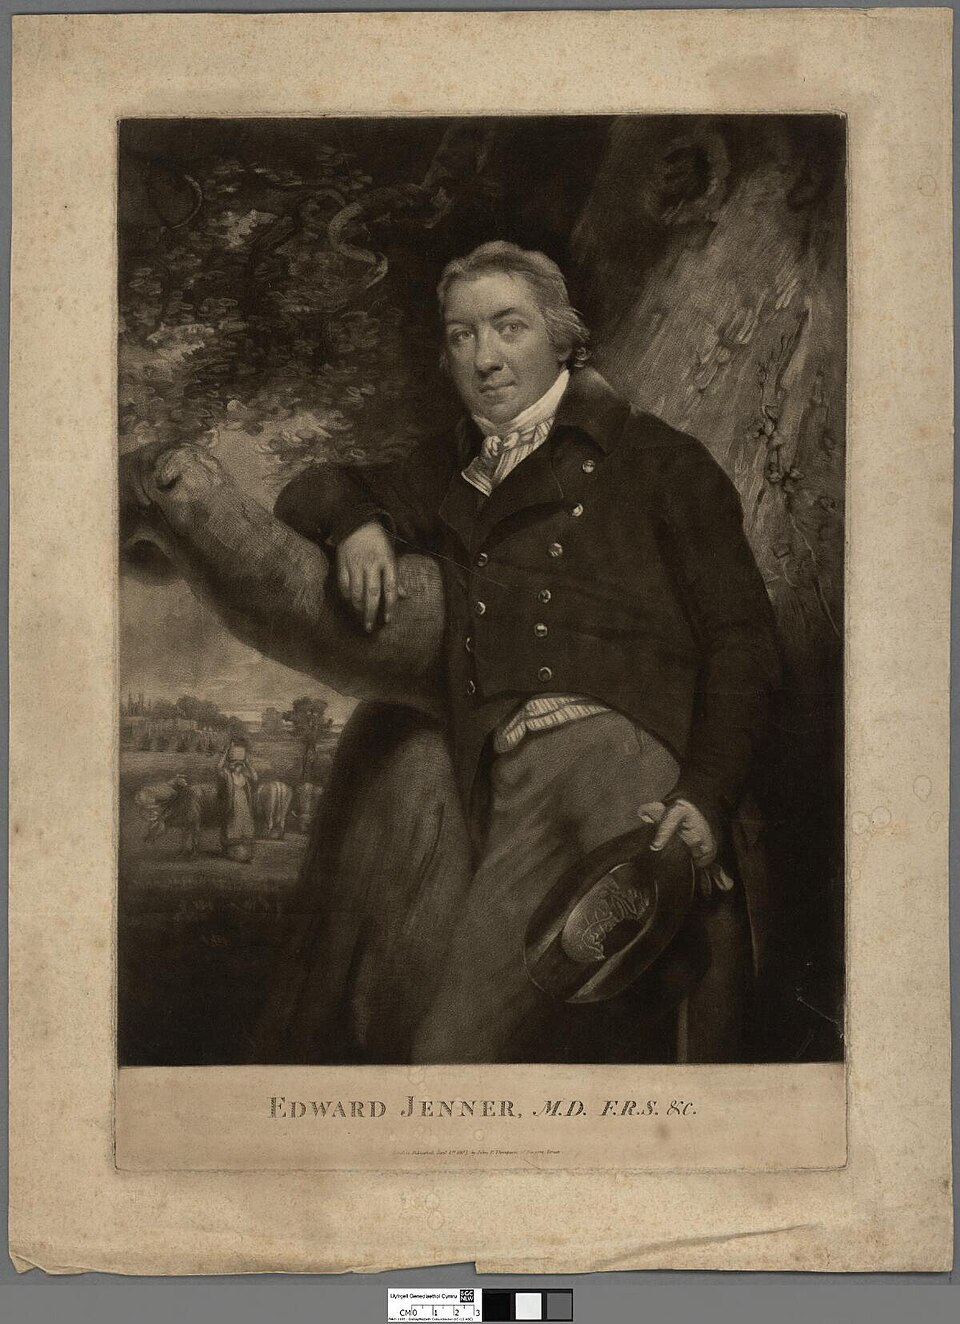
\includegraphics[width=0.30\linewidth]{images/book5/jenner.jpg}\hspace{0.04\linewidth}

\includegraphics[width=0.50\linewidth]{images/book5/ai/b5-16-vaccination.jpg}

{\small 爱德华·詹纳于 1796 年保护了一名男孩免受天花\omterm{def:b3:cancer-biology:metastasis}{侵袭}，
以牛痘为手段，由此创立接种\omterm{def:b3:adaptive-immunity:vaccine}{疫苗}（1807 年版画，公有领域）。右图：两个世纪后的同一行为——
肌内注射的\omterm{def:b3:adaptive-immunity:vaccine}{疫苗}，其\omterm{def:b3:adaptive-immunity:lymphocytes}{抗原}由三角肌的\omterm{def:b3:innate-immunity:innate}{树突状细胞}
携带至腋窝
\omterm{def:b3:adaptive-immunity:lymphocytes}{淋巴结}。}
\end{omfigure}

\begin{remark}[免疫记住了什么]\label{rem:b3:adaptive-immunity:memory}
适应性免疫系统是每个人体内的一台达尔文式机器：
随机变异（V(D)J 重排、\omterm{def:b3:adaptive-immunity:germinal-centre}{体细胞高频突变}）、选择（以\omterm{def:b3:adaptive-immunity:lymphocytes}{抗原}为准，在
\omterm{def:b3:adaptive-immunity:germinal-centre}{生发中心}进行；针对自身，则在\omterm{def:b3:adaptive-immunity:tolerance}{胸腺}中进行）与传承（\omterm{def:b3:adaptive-immunity:response}{记忆细胞}、克隆扩增）。
它在数周之内解决了进化需数千年才能解决的问题：
即一种与此前从未见过的靶标结合的分子，
其解答是直接观察到的进化中研究最为充分的案例之一。
其代价是\omterm{def:b3:adaptive-immunity:tolerance}{自身免疫}；它对\omterm{def:b3:innate-immunity:innate}{先天免疫}判断的依赖是绝对的；而其记忆
（詹纳曾加以利用，\omterm{def:b3:adaptive-immunity:vaccine}{疫苗}则有意将其写入）
正是长寿而繁殖缓慢的动物
得以在快速繁殖的微生物构成的
世界中生存的原因。
\end{remark}

\section{练习}

\begin{exercise}[$\star$]\label{exo:b3:adaptive-immunity:1}
叙述\omterm{def:b3:adaptive-immunity:lymphocytes}{克隆选择}学说的四条基本要点，以及
支持前两条要点各自的实验。
\end{exercise}

\begin{exercise}[$\star$]\label{exo:b3:adaptive-immunity:2}
描述\omterm{def:b3:adaptive-immunity:antibody}{抗体}的结构，并给出
五类\omterm{def:b3:adaptive-immunity:antibody}{抗体}各自的功能。
\end{exercise}

\begin{exercise}[$\star$]\label{exo:b3:adaptive-immunity:3}
比较 MHC~I 类分子与 MHC~II 类分子在细胞
分布、肽段来源、肽段长度，以及识别各自的 T~细胞。
\end{exercise}

\begin{exercise}[$\star$]\label{exo:b3:adaptive-immunity:4}
定义 $R_{0}$ 与\omterm{def:b3:adaptive-immunity:vaccine}{群体免疫}阈值，并计算
流行性腮腺炎（$R_{0} = 5$）、百日咳（$R_{0} = 12$）
及 1918 年流感（$R_{0} = 2.5$）的阈值。
\end{exercise}

\begin{exercise}[$\star\star$]\label{exo:b3:adaptive-immunity:5}
某物种有 $V_{H} = 50$、$D = 20$、$J_{H} = 5$，并有一个单一的
轻链基因座，$V = 60$，$J = 4$。先计算组合库容，再
计入连接因子 $10^{4}$ 后的总库容，并
将其与该动物拥有的 $10^{9}$ 个 B~细胞相比较。
\end{exercise}

\begin{exercise}[$\star\star$]\label{exo:b3:adaptive-immunity:6}
\omterm{def:b3:adaptive-immunity:germinal-centre}{生发中心} B~细胞的可变区长 \qty{1000}{bp}；AID 以每碱基对、
每次分裂 $10^{-3}$ 的速率使其突变。经 $20$ 次分裂后，每个细胞
产生多少次突变？在 $10^{5}$ 个细胞中，共产生多少种
互不相同的单碱基变异\omterm{def:b3:adaptive-immunity:antibody}{抗体}？与 $3000$ 种
可能的单碱基替换相比较。
\end{exercise}

\begin{exercise}[$\star\star$]\label{exo:b3:adaptive-immunity:7}
解释为何一人的 T~细胞不能识别另一人细胞呈递的\omterm{def:b3:virology:virus}{病毒}肽段，
并说明这一事实为何使移植困难，
以及 \omterm{def:b3:adaptive-immunity:mhc}{HLA} 系统为何具有多态性。
\end{exercise}

\begin{exercise}[$\star\star$]\label{exo:b3:adaptive-immunity:8}
预测缺乏下列各项的儿童的免疫表型：(a) RAG1、(b) AIRE、
(c) \omterm{def:b3:adaptive-immunity:tolerance}{FoxP3}、(d) \omterm{def:b3:adaptive-immunity:antibody}{类别转换}酶 AID，以及 (e) CD4 T~细胞。
\end{exercise}

\begin{exercise}[$\star\star$]\label{exo:b3:adaptive-immunity:9}
一种\omterm{def:b3:adaptive-immunity:vaccine}{疫苗}的效力为 \qty{90}{\%}，该疾病的 $R_{0} = 6$。需要多大的
接种覆盖率才能阻断传播？若覆盖率为 \qty{80}{\%}，则
$R_{\text{eff}}$ 为多少，以及一次流行会感染
总人口的多大比例（用末期规模关系，将其中的 $R_{0}$
替换为 $R_{\text{eff}}$，仅作用于易感者——或说明为何
这一做法近似成立）？
\end{exercise}

\begin{exercise}[$\star\star\star$]\label{exo:b3:adaptive-immunity:10}
由 SIR 方程推出定理中的末期规模关系，
并对 $R_{0} = 1.5$、$2$、$3$ 和 $5$ 数值求解。为何
即使不加任何干预，一次流行也从不会感染所有人？
\end{exercise}

\begin{exercise}[$\star\star\star$]\label{exo:b3:adaptive-immunity:11}
\omterm{def:b3:adaptive-immunity:germinal-centre}{亲和力成熟}使结合力在三周内提高一千倍。
将\omterm{def:b3:adaptive-immunity:germinal-centre}{生发中心}视为受选择作用的种群，设
突变率为每个细胞每次分裂 1 次，其中 $10^{-2}$ 的
突变可使亲和力提高 $1.5$ 倍，其余突变为中性或
有害。需要多少轮选择才能使亲和力提高一千倍，
且每轮需筛选多少个细胞？试评述为何
\omterm{def:b3:adaptive-immunity:germinal-centre}{生发中心}以循环方式组织。
\end{exercise}

\begin{exercise}[$\star\star\star$]\label{exo:b3:adaptive-immunity:12}
\omterm{def:b3:adaptive-immunity:tolerance}{自身免疫}病在女性中更为常见，并与 \omterm{def:b3:adaptive-immunity:mhc}{HLA}
等位基因相关；1 型糖尿病在富裕国家的五十年间
增长了五倍。请结合本章及
\cref{ch:b3:microbiomes}中的机制，对每项观察给出解释，并
为每项各设计一项检验。
\end{exercise}

\section{问题：疫苗接种运动}

\begin{problem}[{周末问题——计数库容，测定由 100 个细胞至 1 毫升血清的应答时间，
以进化算法模拟生发中心的运行，
并针对群体免疫阈值规划麻疹接种运动，
最后归结为库容大小、一个浆细胞一天分泌的抗体量，
以及一个国家所需的接种覆盖率}]
\label{pb:b3:adaptive-immunity:1}
数据：$V_{H} = 40$，$D = 25$，$J_{H} = 6$；轻链基因座 $(40, 5)$ 与
$(30, 4)$；连接因子 $3\times 10^{4}$。一个个体有 $10^{11}$
个 B~细胞，其中每 $10^{5}$ 个有一个能结合某一给定表位；$100$ 个前体细胞
被募集，每 \qty{8}{h} 分裂一次，持续 $7$ 天；\qty{30}{\%} 的
克隆细胞变为\omterm{def:b3:adaptive-immunity:response}{浆细胞}，每个\omterm{def:b3:adaptive-immunity:response}{浆细胞}每秒分泌 $2000$ 个 IgG 分子，
IgG 为 \qty{150}{kDa}；血浆体积 \qty{3}{L}；IgG 半衰期
\qty{21}{d}。\omterm{def:b3:adaptive-immunity:germinal-centre}{生发中心}：可变区 \qty{1000}{bp}，$10^{-3}$
每碱基对每次分裂的突变数，$100$ 个突变中有一个可使
亲和力提高 $1.5$ 倍。麻疹：$R_{0} = 15$，\omterm{def:b3:adaptive-immunity:vaccine}{疫苗效力}为 $0.93$（接种一剂后）；
接种两剂后为 $0.97$；一个国家
人口 $5\times 10^{6}$，每年出生 $60\,000$ 人。

\medskip
\noindent\textbf{第一部分——库容。}
\begin{enumerate}
  \item 计算组合库容，以及计入
        \omterm{def:b3:adaptive-immunity:antibody}{连接多样性}后的总库容。
  \item 与 B~细胞数相比较。一个个体同一时刻表达的
        库容占可能库容的多大比例，
        由此对两个个体的库容可得出什么结论？
  \item 体内有多少 B~细胞能结合该表位？其中平均
        在含 $10^{8}$ 个 B~细胞的\omterm{def:b3:adaptive-immunity:lymphocytes}{淋巴结}中有多少个？
  \item 新生儿有 $10^{9}$ 个 B~细胞。其中有多少个能结合该表位，
        新生儿的应答为何即便如此仍较弱？
  \item \omterm{def:b3:adaptive-immunity:antibody}{抗体}重链第三个环由\omterm{def:b3:adaptive-immunity:antibody}{连接多样性}产生。试说明为何该环
        是分子中变异最大的部分，
        且通常位于结合位点的中心。
  \item \omterm{def:b3:adaptive-immunity:germinal-centre}{体细胞高频突变}在选择之后增加多样性，V(D)J 重组则在选择之前。
        为何两者都具备，且按此顺序出现，是有利的？
\end{enumerate}

\medskip
\noindent\textbf{第二部分——应答。}
\begin{enumerate}[resume]
  \item 从 $100$ 个每 \qty{8}{h} 分裂一次的细胞出发，经 $7$
        天后共有多少个细胞？其中有多少个为\omterm{def:b3:adaptive-immunity:response}{浆细胞}？
  \item 它们每天分泌多少个 IgG 分子，质量
        为多少？一天的分泌量在
        \qty{3}{L} 中产生的血清浓度为多少？
  \item 若以该速率分泌十天并忽略衰减，
        其浓度为多少 g/L？与正常的 IgG 总量
        \qty{10}{g/L} 相比如何？
  \item \omterm{def:b3:adaptive-immunity:response}{浆细胞}两周后死亡，此后\omterm{def:b3:adaptive-immunity:antibody}{抗体}以
        半衰期 \qty{21}{d} 衰减。第 9 题中的浓度需要多长时间
        才会降至百分之一？什么维持了\omterm{def:b3:adaptive-immunity:antibody}{抗体}
        数年之久的水平？
  \item 二次应答从 $10^{5}$ 个\omterm{def:b3:adaptive-immunity:response}{记忆细胞}开始，
        经 $3$ 天后共有多少个细胞？这与初次应答
        在第 3 天和第 7 天的情况相比如何？
  \item 解释为何初次应答中 IgM 先出现、IgG 后出现，
        以及为何二次应答一开始即为 IgG。
\end{enumerate}

\medskip
\noindent\textbf{第三部分——\omterm{def:b3:adaptive-immunity:germinal-centre}{生发中心}。}
\begin{enumerate}[resume]
  \item 一个 B~细胞的可变区每次分裂获得多少个突变，
        $20$ 次分裂后共有多少个？
  \item 一次分裂的子代中，携带改善亲和力
        突变的比例为多少？在含 $10^{4}$ 个分裂细胞的
        \omterm{def:b3:adaptive-immunity:germinal-centre}{生发中心}中，每次分裂出现多少个亲和力提高的细胞？
  \item 连续多少次各提高 $1.5$ 倍，才能
        使亲和力提高一千倍？若每轮选择需两次分裂，
        即 \qty{12}{h}，则共需多长时间？
  \item 多数突变会损害\omterm{def:b3:adaptive-immunity:antibody}{抗体}。若 \qty{50}{\%} 的突变
        破坏结合能力，则每次分裂后经突变仍存活的
        细胞比例为多少？为何明区必须淘汰大多数细胞？
  \item 相隔六周接种两剂的\omterm{def:b3:adaptive-immunity:vaccine}{疫苗}，所产生的\omterm{def:b3:adaptive-immunity:antibody}{抗体}
        亲和力高于单剂，试结合\omterm{def:b3:adaptive-immunity:germinal-centre}{生发中心}
        加以解释。
  \item 某些\omterm{def:b3:virology:virus}{病毒}（HIV、流感\omterm{def:b3:virology:virus}{病毒}）通过突变其
        表面以逃避\omterm{def:b3:adaptive-immunity:antibody}{抗体}。试解释为何\omterm{def:b3:adaptive-immunity:germinal-centre}{生发中心}仍是
        广谱保护性\omterm{def:b3:adaptive-immunity:vaccine}{疫苗}的希望所在。
\end{enumerate}

\medskip
\noindent\textbf{第四部分——接种行动。}
\begin{enumerate}[resume]
  \item 麻疹的\omterm{def:b3:adaptive-immunity:vaccine}{群体免疫}阈值，以及单剂
        接种所需的覆盖率，以及两剂接种所需的覆盖率。
  \item 某国以两剂\omterm{def:b3:adaptive-immunity:vaccine}{疫苗}接种了 \qty{90}{\%} 的儿童。
        求免疫人口比例与 $R_{\text{eff}}$，并判断
        麻疹能否继续传播？
  \item 每年出生的儿童在
        \qty{90}{\%} 的接种率下，累积多少易感儿童（未接种者加上接种失败者）？
        此后五年无麻疹，易感者有多少，
        为何此时一次输入性病例会引发暴发？
  \item 利用终末规模关系式，
        结合易感人群中的有效再生数，估计一次暴发
        在这些易感者中感染的比例。（取问题 20 中的
        $R_{\text{eff}}$ 作为全人群的再生数，并注意
        在易感人群中，疾病的传播如同 $R_{0}$ 等于
        $R_{\text{eff}}$ 一样进行。）
  \item 若两剂接种的覆盖率提高至 \qty{95}{\%}，求
        免疫人口比例与 $R_{\text{eff}}$，阈值是否达到？
  \item 不满一岁的婴儿不能接种麻疹\omterm{def:b3:adaptive-immunity:vaccine}{疫苗}，
        却最容易因此死亡。试说明接种行动如何
        保护他们，以及若接种率
        降至 \qty{85}{\%}，他们的保护情况会怎样？
  \item 试作总结：全部库容（问题~1）、一天之内\omterm{def:b3:adaptive-immunity:response}{浆细胞}所产生的
        IgG（问题~8）以及该国所需的两剂接种覆盖率
        （问题~19）。
\end{enumerate}
\end{problem}
